\section{4点関数}

この節では強結合領域$\beta J \gg 1$における4点関数を論じる。
disorder-averageを取る事によって最も一般的な4点関数は
\begin{align}
	\average{\psi_i(t_1)\psi_i(t_2)\psi_j(t_3)\psi_j(t_4)}
\end{align}
という形に制限される。
これを$i$と$j$について平均を取ったものを考える:
\begin{align}
	\frac{1}{N^2}\sum_{i,j=1}^{N}\average{T\psi_i(t_1)\psi_i(t_2)\psi_j(t_3)\psi_j(t_4)}
	= G(t_{12})G(t_{34}) + \frac{1}{N}\mathcal{F}(t_1, \cdots, t_4).
	\label{eq:fourpointfunc}
\end{align}
以下では$\mathcal{F}$について解析する。

\begin{figure}[h]
	\centering
	\vspace{1cm}
	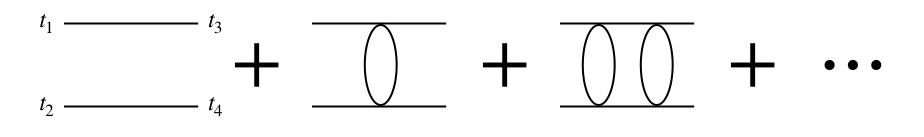
\includegraphics[width=13cm]{figures/ladderDiagram}
	\caption{\eqref{eq:fourpointfunc}式の$1/N$の項を表すダイアグラム。
		特に$q=4$の場合について描画した。ラダーダイアグラムと呼ぶ。}
	\label{fig:ladderdiagram}
\end{figure}

$\mathcal{F}$を表すダイアグラムはラダーダイアグラムである(図\ref{fig:ladderdiagram})。
$n$個の輪があるものを$\mathcal{F}_n$とすると、計算するべきは
\begin{align}
	\mathcal{F} = \sum_n \mathcal{F}_n
\end{align}
である。
図\ref{fig:ladderdiagram}の最初にある輪を持たないラダーダイアグラムは単なるプロパゲーターの積である:
\begin{align}
	\mathcal{F}_0(t_1, \cdots, t_4) = -G(t_{13})G(t_{24}) + G(t_{14})G(t_{23}).
\end{align}
次に並ぶ、輪を1個だけ持つラダーダイアグラムでは、輪の端の位置について積分した形で与えられる:
\begin{align}
	\mathcal{F}_1(t_1, &\cdots, t_4)\nonumber\\
	&= J^2(q - 1)\int dtdt'\ \left(
		G(t_1 - t)G(t_2 - t')G(t - t')^{q-2}G(t - t_3)G(t' - t_4) - (t_3 \leftrightarrow t_4)
	\right).
\end{align}
積分の前にある$q-1$という因子は、どの線をレールや輪にするかのパターン数に起因する。
上述した2つのラダーダイアグラム$\mathcal{F}_0$、$\mathcal{F}_1$に限らず、
全てのラダーダイアグラムは$1/N$に比例する。

あるラダーダイアグラム$\mathcal{F}_n$と次の$\mathcal{F}_{n+1}$の間には
\begin{align}
	\mathcal{F}_{n+1}(t_1, \cdots, t_4)
	= \int dtdt'\ K(t_1, t_2; t, t')\mathcal{F}_n(t, t', t_3, t_4)
	\label{eq:F_n+1_and_F_n}
\end{align}
という漸化式的な関係がある。
ここで積分核$K$は
\begin{align}
	K(t_1, t_2; t_3, t_4) = -J^2(q-1)G(t_{13})G(t_{24})G(t_{34})^{q-2}
	\label{eq:def_of_K}
\end{align}
である。
\eqref{eq:F_n+1_and_F_n}式の計算では、$K$の最初の2つの変数を1つめの添字、残りの2つを2つ目の添字
と見なす事によって積分を行列計算としてしまうのが便利である(行列$K$は2変数反対称関数の空間に作用する)。
こうする事で全てのラダーダイアグラムの総和を
\begin{align}
	\mathcal{F}
	= \sum_{n=0}^{\infty}\mathcal{F}_n
	= \sum_{n=0}^{\infty}K^n \mathcal{F}_0
	= \frac{1}{1 - K}\mathcal{F}_0
	\label{eq:geometric_series_of_F}
\end{align}
という様に表す事ができる。
これを更に計算するために、以下では$K$を対角化する事を考える。
\eqref{eq:def_of_K}式による定義では$K$は対称行列ではないが、
次のような操作により対称化する事が可能である:
\begin{align}
	\tilde{K}(t_1, t_2; t_3, t_4) \equiv
	|G(t_{12})|^{\frac{q-2}{2}}K(t_1, t_2; t_3, t_4)|G(t_{34})|^{\frac{2-q}{2}}.
\end{align}
従って$K$は固有関数(固有ベクトル)の完全系を持つとして良い。

\subsection{$K_c$の対角化}
ここまでの話は一般の$\beta J$について成り立つ。
解析を進めるために、以下では共形対称性の成り立つ極限$\beta J \gg 1$で考える。
よって2点関数は$\eqref{eq:conformal_ansatz}$式の$G_c(t)$で与えられる。
\eqref{eq:conformal_ansatz}式を\eqref{eq:def_of_K}式に代入すると、
$K$の共形不変なものとして
\begin{align}
	K_c(t_1, t_2; t_3, t_4)
	= -\frac{1}{\alpha_0}
		\frac{\sgn(t_{13})\sgn(t_{24})}{|t_{13}|^{2\Delta}|t_{24}|^{2\Delta}|t_{34}|^{2-4\Delta}}
	\label{eq:confomarl_K}
\end{align}
を得る。ここで
\begin{align}
	\alpha_0 \equiv \frac{2\pi q}{(q-1)(q-2)\tan\frac{\pi}{q}}
\end{align}
である。
$K_c$を対角化した暁には、実は固有関数の中に固有値$g(\alpha) = 1$を持つものも存在する。
従って\eqref{eq:geometric_series_of_F}式の級数は発散するが、これは共形極限から摂動的に少し
ずれる事によって対処する事ができる。
それを議論するまでは、ひとまず\eqref{eq:confomarl_K}式を用いる事にする。

$K_c$の対角化では共形不変性を活用する事になる。
SYK模型は時間1次元しか持たないので、1次元共形場理論$\mathrm{CFT}_1$であり
\footnote{1次元の場の量子論は本質的に量子力学なので、
Conformal Quantum Mechanicsの頭文字を取ってCQMと表記する事もある。}、
共形変換群は$SL(2, \mathbb{R})$で与えられる\cite{andrzejewski}:
\begin{align}
	\hat{D} = -t\partial_t - \Delta,\hspace{20pt}
	\hat{P} = \partial_t,\hspace{20pt}
	\hat{K} = t^2\partial_t + 2t\Delta,
\end{align}
\begin{align}
	[\hat{D}, \hat{P}] = \hat{P},\hspace{20pt}
	[\hat{D}, \hat{K}] = -\hat{K},\hspace{20pt}
	[\hat{P}, \hat{K}] = -2\hat{D}.
\end{align}
これらの生成子は$K_c$と交換し、
\begin{align}
	(\hat{D}_1 + \hat{D}_2)K_c(t_1, t_2; t_3, t_4)
	= K_c(t_1, t_2; t_3, t_4)(\hat{D}_3 + \hat{D}_4)
\end{align}
となる。$\hat{P}$や$\hat{K}$についても同様である。
この対称性により、まずラダーダイアグラム$\mathcal{F}_n$は$SL(2, \mathbb{R})$不変の
断面比(cross ratio)
\begin{align}
	\chi = \frac{t_{12}t_{34}}{t_{13}t_{24}}
\end{align}
の関数である事が示唆される。
これは$\mathcal{F}_0$が共形4点関数のように変換するからである。
この性質は$SL(2, \mathbb{R})$不変の演算子を作用させても変わらない。
従って$K_c(t_1, t_2; t_3, t_4)$とする代わりに$K_c(\chi; \tilde{\chi})$とする事ができる。
2つ目の示唆は、$K_c$が次式で与えられるカシミール演算子$C_{1+2}$と可換というものである:
\begin{align}
	C_{1+2}
	&= (\hat{D}_1 + \hat{D}_2)^2
	- \frac{1}{2}(\hat{K}_1 + \hat{K}_2)(\hat{P}_1 + \hat{P}_2)
	- \frac{1}{2}(\hat{P}_1 + \hat{P}_2)(\hat{K}_1 + \hat{K}_2)\nonumber\\
	&= 2(\Delta^2 - \Delta) - \hat{K}_1\hat{P}_2 - \hat{P}_1\hat{K}_2 + 2\hat{D}_1\hat{D}_2.
\end{align}
スペクトラムに縮退はないため、これは$K_c$の固有関数が$C_{1+2}$のそれと同じである事を意味する。
\eqref{eq:geometric_series_of_F}式を$C_{1+2}$の固有関数$\Psi_h(\chi)$で展開すれば、
何らかの内積を用いて
\begin{align}
	\mathcal{F}(\chi)
	= \sum_h \Psi_h(\chi)\frac{1}{1 - k_c(h)}
		\frac{\innerprod{\Psi_h}{\mathcal{F}_0}}{\innerprod{\Psi_h}{\Psi_h}}
\end{align}
と変形できる。
よって我々が行うべき仕事は$\Psi_h$と$k_c(h)$を求め、そして内積を計算する事である。
そのために、まず$\chi$の関数としての$\mathcal{F}_n$の性質を調べる事から始める。

\subsubsection{$\mathcal{F}_n(\chi)$の性質}
共形極限では、ラダーダイアグラム$\mathcal{F}_n$は$SL(2, \mathbb{R})$変換のもとで
次元$\Delta$を持つ4点関数として振る舞う:
\begin{align}
	\mathcal{F}_n(t_1, t_2; t_3, t_4)
	= G_c(t_{12})G_c(t_{34})\mathcal{F}_n(\chi).
\end{align}
$t_1$と$t_2$の間、および$t_3$と$t_4$の間の反対称性、さらに$(t_1, t_2)$と$(t_3, t_4)$の間の対称性
や$SL(2, \mathbb{R})$変換を駆使すると、$t_1 = 0$、$t_3 = 1$、$t_4 = \infty$さらに$t_2 > 0$
という様に移す事ができ、$\chi = t_2$の値を正であるとして制限できる。
\eqref{eq:fourpointfunc}式の時間順序積の存在により、$\chi > 1$か$\chi < 1$かによって
\begin{align}
	\mathcal{F}_n(\chi)
	\approx \left\{
		\begin{array}{l}
			+\average{\psi_j(\infty)\psi_j(1)\psi_i(\chi)\psi_i(0)}\hspace{20pt}
			0 < \chi < 1\\
			-\average{\psi_j(\infty)\psi_i(\chi)\psi_j(1)\psi_i(0)}\hspace{20pt}
			1 < \chi < \infty
		\end{array}
	\right.
\end{align}
となる。

$\chi > 1$の領域では、ある離散的な対称性が存在する。
これを見るには
\begin{align}
	\frac{t-2}{t} = \tan \frac{\theta}{2}
\end{align}
として$t$を円周上に写像すると良い。
$t = 0, 1, \infty$はそれぞれ$\theta = -\pi, -\frac{\pi}{2}, \frac{\pi}{2}$に写される。
$t_2 = \chi$はある$\theta$が対応する。

\pagebreak
